\section{Pengembangan Prototipe \textit{Low-Fidelity}}
\label{sec:lofi}

Prototipe \textit{Low-Fidelity} adalah sebuah cara yang efektif untuk merealisasi rancangan solusi dari sebuah desain beserta dengan konsep-konsep desain menjadi sebuah artefak yang dapat dilakukan interaksi oleh pengguna produknya. \parencite{adobe2017prototype} Tujuan dari pembuatan prototipe \textit{low-fidelity} adalah untuk merealisasikan fungsionalitas inti dari produk sehingga tersampaikan kepada pengguna, sebelum mengikutsertakan elemen-elemen visual lainnya. 

\newpage

\subsection{Perancangan Navigasi Prototipe}
\label{subsec:lofi_navigasi}
Perlu dibentuk rancangan navigasi yang akan menghubungkan halaman-halaman yang telah ditentukan pada Tabel \ref{tab:daftar_halaman}. Pada Gambar \ref{fig:diagram_navigasi} dapat ditemukan Diagram Navigasi yang menggambarkan hubungan interaksi antarhalaman dari prototipe. Hal ini akan menjadi salah satu dari acuan pengujian prototipe \textit{low-fidelity}.
Perlu diingat bahwa widget akan diimplementasikan dalam prototipe, namun widget tidak dapat diakses langsung dari aplikasi melainkan perlu ditambahkan ke dalam Homescreen dari \textit{smartphone}, sehingga widget tidak termasuk ke dalam Diagram Navigasi.  

\newpage

\begin{landscape}
  \begin{figure}[h]
    \centering
    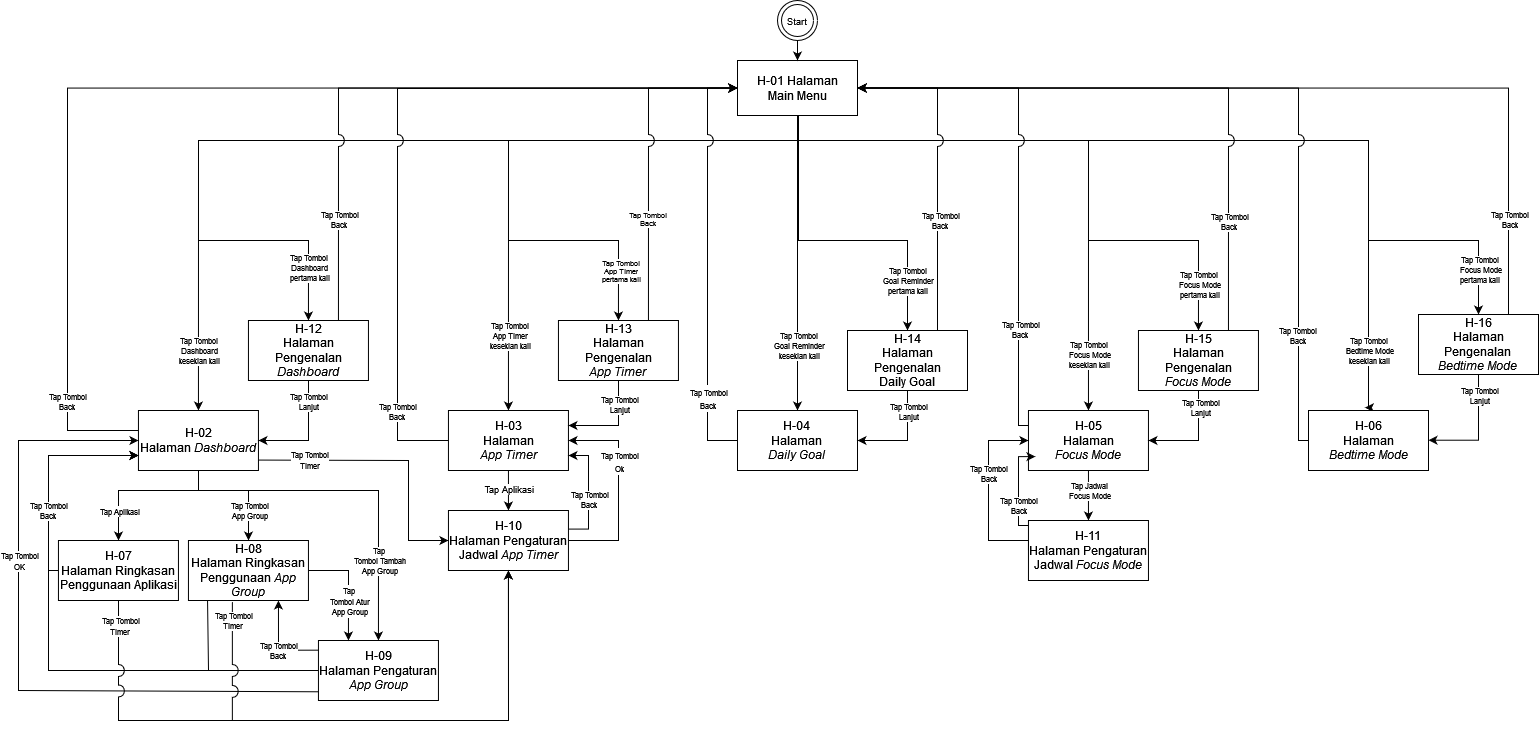
\includegraphics[width=1.7\textwidth]{chapter-4-diagram-navigasi.png}
    \caption{Diagram Navigasi}
    \label{fig:diagram_navigasi}
  \end{figure}
\end{landscape}

\newpage


\subsection{Implementasi Prototipe \textit{Low-Fidelity}}
\label{subsec:lofi_implementasi}
Tampilan dari halaman serta widget yang telah ditentukan perlu memuat informasi dan elemen interaksi yang cukup bagi pengguna untuk mencapai tujuannya saat menggunakan prototipe \textit{low-fidelity}. Tabel \ref{tab:daftar_lofi_halaman} memuat implementasi tampilan halaman prototipe \textit{low-fidelity}, sedangkan Tabel \ref{tab:daftar_lofi_widget} memuat implementasi tampilan untuk widget. Pada kedua tabel tersebut dimuat juga pemetaan beberapa prinsip desain yang telah disebutkan pada Tabel \ref{tab:prinsip_desain} terhadap prototipe \textit{low-fidelity}, serta penjelasan singkat tentang tampilan.

\newpage


\newlength{\lofiwidth}
\setlength{\lofiwidth}{0.325\textwidth}


\newlength{\lofidescwidth}
\setlength{\lofidescwidth}{0.35\textwidth}

\newcommand{\desc}[2]{\begin{minipage}[t]{#1}\linespread{1.0}\selectfont{#2}\end{minipage}}
\newcommand{\lofidesc}[1]{\desc{\lofidescwidth}{#1}}

\newcommand{\lofi}[1]{\begin{center}\includegraphics[width=\lofiwidth]{#1}\end{center}}
\newcommand{\lofiwidget}[2]{\begin{center}\includegraphics[width=#1]{#2}\end{center}}

\RaggedLeft
\begin{footnotesize}
\begin{longtable}[c]{|>{\ccnormspacingcenter}p{0.12\textwidth}|>{\ccnormspacing}p{\lofidescwidth}|>{\ccnormspacingcenter}p{0.1\textwidth}|>{\ccnormspacingcenter}p{\lofiwidth}|}
  \caption{Daftar Tampilan Halaman Prototipe \textit{Low-Fidelity}}
  \label{tab:daftar_lofi_halaman} \\
  \hline \rowcolor[HTML]{A3E5F5}
  \centering\textbf{Halaman} & \centering\textbf{Penjelasan Halaman} & \centering\textbf{Prinsip Desain} & \textbf{Prototipe \textit{Low-Fidelity}} \\ \hline \endfirsthead
  \hline \rowcolor[HTML]{A3E5F5}
  \centering\textbf{Halaman} & \centering\textbf{Penjelasan Halaman} & \centering\textbf{Prinsip Desain} & \textbf{Prototipe \textit{Low-Fidelity}} \\ \hline \endhead
  \hline \endfoot

  \textbf{H-01} Halaman Main Menu & 
    \lofidesc{
      Halaman ini adalah tampilan utama dari aplikasi Digital Wellbeing yang memuat navigasi utama ke fitur-fitur seperti Dashboard, App Timer, Daily Goal, Focus Mode, dan Bedtime Mode. Navigasi menuju Dashboard diletakkan di paling atas beserta \textit{pie graph} yang menunjukkan aktivitas \textit{smartphone} pengguna di hari tersebut. Di bagian bawah juga terdapat navigasi menuju pengaturan notifikasi dan mode "Do Not Disturb" bawaan \textit{smartphone}
    } & DP-01, DP-02, DP-04, DP-05, DP-08, DP-09 & \lofi{lofi/h-01} \\ \hline

  \textbf{H-02} Halaman Dashboard & 
  \lofidesc{
    Halaman ini memuat seluruh data penggunaan \textit{smartphone}. Pada bagian paling atas, terdapat rekomendasi dari Digital Wellbeing tentang langkah-langkah yang dapat dilakukan pengguna untuk memperbaiki kebiasaan digitalnya, atau penanda jika kebiasaannya sudah cukup sehat. Bagian rekomendasi ini adalah salah satu aspek di mana tipe interaksi \textit{responding} difokuskan. Data penggunaan \textit{smartphone} yang ditampilkan dapat dipilih oleh menu, baik waktu penggunaan aplikasi, jumlah notifikasi, atau jumlah pembukaan aplikasi. Periode durasi data juga dapat dipilih dengan menu, baik secara per jam, harian, atau mingguan. \newline
    Selain itu terdapat daftar seluruh aplikasi pada \textit{smartphone} beserta data penggunaannya masing-masing. Pengguna dapat melihat data lebih detail atau langsung memasang App Timer. Pengguna juga dapat melihat data penggunaan dari kelompok aplikasi yang telah dibuat, atau membuatnya jika belum ada, terlihat tepat di atas daftar. Jika pengguna ingin mencari aplikasi spesifik, maka \textit{searchbar} bisa dimanfaatkan untuk mengetikkan nama aplikasi.
  } & DP-01, DP-02, DP-03, DP-04, DP-05, DP-08, DP-09 & \lofi{lofi/h-02} \\ \hline

  \textbf{H-03} Halaman App Timer & 
    \lofidesc{
      Halaman ini berisi daftar App Timer yang telah dipasang oleh pengguna, waktu yang telah dilampaui selama menggunakan aplikasi tersebut, serta sisa waktu sebelum aplikasi ditutup aksesnya. Pengguna bisa mengubah pengaturan App Timer yang telah dipasang, atau menambah aplikasi atau App Group yang ingin dipasangkan App Timer dengan mencarinya dari daftar aplikasi yang terletak di bawah. Di halaman ini pengguna juga bisa mengatur perilaku pemberian peringatan terhadap sisa waktu aplikasi-aplikasi.
    } & DP-02, DP-03, DP-05, DP-08, DP-09 & \lofi{lofi/h-03} \\ \hline
  
  \textbf{H-04} Halaman Daily Goal & 
    \lofidesc{
      Di halaman ini, pengguna dapat menentukan Daily Goal atau tujuan harian yang ingin ditempuh dan dibantu diingatkan oleh aplikasi Digital Wellbeing. Pengguna dapat mengatur perilaku pengiriman peringatannya. Pengguna juga dapat menyalakan fitur Smartphone Usage Evaluation di mana aplikasi akan mengirimkan sebuah notifikasi berisi jumlah waktu penggunaan \textit{smartphone} pada hari tersebut serta peringatan untuk mengevaluasi Daily Goal yang telah ditentukan.
    } & DP-03, DP-05, DP-06, DP-08, DP-09 & \lofi{lofi/h-04} \\ \hline
  
  \textbf{H-05} Halaman Focus Mode & 
    \lofidesc{
      Halaman ini memuat status dari keberjalanan Focus Mode serta aksi-aksi yang dapat dilakukan untuk menunda, mematikan, atau mengaktivasinya. Selain itu, terdapat juga daftar jadwal Focus Mode yang ditentukan pengguna, atau pilihan untuk menambahkannya. Jadwal Focus Mode akan menavigasikan pengguna ke halaman pengaturan jadwal tersebut.
    } & DP-03, DP-05, DP-06, DP-08, DP-09 & \lofi{lofi/h-05} \\ \hline
  
  \textbf{H-06} Halaman Bedtime Mode & 
    \lofidesc{
      Pada halaman ini, pengguna dapat mengatur jadwal aktivasi Bedtime Mode menurut mode perilaku aktivasi yang dipilihnya. Pengguna juga dapat mengatur kemampuan apa saja yang akan aktif jika Bedtime Mode berlangsung.
    } & DP-03, DP-04, DP-05, DP-08, DP-09 & \lofi{lofi/h-06-schedule} \\ \hline
  
  \textbf{H-07} Halaman Ringkasan Penggunaan Aplikasi & 
    \lofidesc{
      Halaman ini memuat data penggunaan sebuah aplikasi. Jenis data-data yang ditampilkan mirip seperti yang dapat ditemukan pada halaman Dashboard, namun hanya untuk satu buah aplikasi yang dipilih saja. Pemilihan periode waktu serta navigasi waktu data juga dapat dilakukan. Sebagai tambahan, terdapat navigasi ke halaman pengaturan App Timer untuk aplikasinya, serta navigasi menuju halaman pengaturan notifikasi aplikasi bawaan \textit{smartphone}. Tampilan data penggunaan aplikasi sengaja dibuat serupa dengan tampilan pengguna \textit{smartphone} agar pengguna dapat dengan mudah menggunakannya tanpa perlu mempelajari ulang.
    } & DP-05, DP-08, DP-09 & \lofi{lofi/h-07} \\ \hline
  
  \textbf{H-08} Halaman Ringkasan Penggunaan App Group & 
    \lofidesc{
      Halaman ini memuat data penggunaan dari App Group atau kelompok aplikasi yang ditentukan oleh pengguna. Jenis data-data yang ditampilkan mirip seperti yang dapat ditemukan pada halaman Dashboard, namun hanya untuk gabungan dari beberapa aplikasi yang ditentukan. Pemilihan periode waktu serta navigasi waktu data juga dapat dilakukan. Di bagian bawah, terdapat daftar aplikasi yang termasuk ke dalam App Group, yang dapat dinavigasi ke halaman data penggunaan aplikasinya masing-masing, atau halaman pengaturan App Timer aplikasinya. Sebagai tambahan, terdapat juga navigasi ke halaman App Timer untuk App Group tersebut, di mana dapat diatur App Timer untuk keseluruhan aplikasi secara kolektif. Terdapat juga navigasi ke halaman pengaturan App Group jika pengguna ingin melakukan perubahan.
    } & DP-05, DP-08, DP-09 & \lofi{lofi/h-08} \\ \hline
  
  \textbf{H-09} Halaman Pengaturan App Group & 
    \lofidesc{
      Pada halaman ini dapat dilakukan pengaturan terhadap App Group yang dibuat oleh pengguna. Pengaturan App Group termasuk nama App Group serta aplikasi-aplikasi yang dipilih. Pengguna dapat memanfaatkan \textit{searchbar} jika ingin mencari aplikasi yang spesifik.
    } & DP-05, DP-08, DP-09 & \lofi{lofi/h-09} \\ \hline
  
  \textbf{H-10} Halaman Pengaturan Jadwal App Timer & 
    \lofidesc{
      Pada halaman ini dapat dilakukan pengaturan terhadap App Timer aplikasi yang dibuat oleh pengguna. Pengguna dapat mengatur App Timer agar memiliki batas waktu yang sama setiap hari, atau batas waktu yang berbeda-beda per harinya sesuai kebutuhan pengguna. Pengguna juga dapat menghapus App Timer lewat halaman ini. Di bagian atas juga terdapat visualisasi waktu penggunaan aplikasi dan sisa batas waktunya untuk hari tersebut.
    } & DP-01, DP-02, DP-03, DP-05, DP-08, DP-09 & \lofi{lofi/h-10-custom} \\ \hline
  
  \textbf{H-11} Halaman Pengaturan Jadwal Focus Mode & 
    \lofidesc{
      Pada halaman ini, pengguna dapat mengatur hari dan waktu aktivasi dari jadwal Focus Mode yang dibuat pengguna. Pengguna juga dapat mengatur nama dari jadwal, dan aplikasi apa saja yang akan diblokir aksesnya selama jadwal Focus Mode berlangsung. Jika pengguna ingin mencari aplikasi spesifik, maka \textit{searchbar} dapat dimanfaatkan dengan mengetikkan nama aplikasinya.
    } & DP-03, DP-05, DP-08, DP-09 & \lofi{lofi/h-11} \\ \hline
  
  
  \textbf{H-12} Halaman Pengenalan Dashboard & 
    \lofidesc{
      Halaman ini memuat ilustrasi tujuan dari Dashboard dan penjelasan tentang fitur-fitur yang terdapat pada Dashboard. Halaman ini bertujuan agar pengguna memiliki gambaran umum tentang apa yang dapat dicapai dari menggunakan Dashboard.
    } & DP-05, DP-09 & \lofi{lofi/h-12} \\ \hline
  
  \textbf{H-13} Halaman Pengenalan App Timer & 
    \lofidesc{
      Halaman ini memuat ilustrasi tujuan dari App Timer dan penjelasan tentang fitur-fitur yang terdapat pada App Timer. Halaman ini bertujuan agar pengguna memiliki gambaran umum tentang apa yang dapat dicapai dari menggunakan App Timer.
    } & DP-05, DP-09 & \lofi{lofi/h-13} \\ \hline
  
  \textbf{H-14} Halaman Pengenalan Goal Reminder & 
    \lofidesc{
      Halaman ini memuat ilustrasi tujuan dari Daily Goal dan penjelasan tentang fitur-fitur yang terdapat pada Daily Goal. Halaman ini bertujuan agar pengguna memiliki gambaran umum tentang apa yang dapat dicapai dari menggunakan Daily Goal.
    } & DP-05, DP-09 & \lofi{lofi/h-14} \\ \hline
  
  \textbf{H-15} Halaman Pengenalan Focus Mode & 
    \lofidesc{
      Halaman ini memuat ilustrasi tujuan dari Focus Mode dan penjelasan tentang fitur-fitur yang terdapat pada Focus Mode. Halaman ini bertujuan agar pengguna memiliki gambaran umum tentang apa yang dapat dicapai dari menggunakan Focus Mode.
    } & DP-05, DP-09 & \lofi{lofi/h-15} \\ \hline
  
  \textbf{H-16} Halaman Pengenalan Bedtime Mode & 
    \lofidesc{
      Halaman ini memuat ilustrasi tujuan dari Bedtime Mode dan penjelasan tentang fitur-fitur yang terdapat pada Bedtime Mode. Halaman ini bertujuan agar pengguna memiliki gambaran umum tentang apa yang dapat dicapai dari menggunakan Bedtime Mode
    } & DP-05, DP-09 & \lofi{lofi/h-16} \\ \hline


\end{longtable}
\end{footnotesize}
\justifying
\FloatBarrier

\RaggedLeft
\begin{footnotesize}
\begin{longtable}[c]{|>{\ccnormspacingcenter}p{0.1\textwidth}|>{\ccnormspacing}p{0.35\textwidth}|>{\ccnormspacingcenter}p{0.11\textwidth}|>{\ccnormspacingcenter}p{\lofiwidth}|}
  \caption{Daftar Tampilan Widget Prototipe \textit{Low-Fidelity}}
  \label{tab:daftar_lofi_widget} \\
  \hline \rowcolor[HTML]{A3E5F5}
  \centering\textbf{Widget} & \centering\textbf{Penjelasan Widget} & \centering\textbf{Prinsip Desain} & \textbf{Prototipe \textit{Low-Fidelity}} \\ \hline \endfirsthead
  \hline \rowcolor[HTML]{A3E5F5}
  \centering\textbf{Widget} & \centering\textbf{Penjelasan Widget} & \centering\textbf{Prinsip Desain} & \textbf{Prototipe \textit{Low-Fidelity}} \\ \hline \endhead
  \hline \endfoot

  \textbf{W-01} Widget Dashboard & 
    \lofidesc{
      Widget ini memuat data penggunaan \textit{smartphone}, serta 3 aplikasi dengan penggunaan tertinggi pada hari tersebut. Pengguna dapat melakukan navigasi langsung ke halaman Dashboard melalui widget ini.
    } & DP-02, DP-05, DP-09 & \lofiwidget{0.2\textwidth}{lofi/w-01} \\ \hline

  \textbf{W-02} Widget App Timer & 
    \lofidesc{
      Widget ini memuat daftar aplikasi yang telah dipasang App Timer, serta sisa waktu untuk menggunakan aplikasi sebelum aksesnya ditutup. Pengguna dapat melakukan navigasi langsung ke halaman App Timer, atau menambah App Timer untuk aplikasi lain melalui widget ini.
    } & DP-02, DP-05, DP-09 & \lofiwidget{0.3\textwidth}{lofi/w-02} \\ \hline
 
  \textbf{W-03} Widget Focus Mode & 
    \lofidesc{
      Widget ini menampilkan status keberlangsungan dari Focus Mode. Pengguna dapat mengaktivasi Focus Mode langsung dari widget jika sedang tidak aktif, serta mengambil istirahat dan mematikan Focus Mode jika sedang aktif. Pengguna juga dapat melakukan navigasi langsung ke halaman Focus Mode langsung dari widget.
    } & DP-03, DP-04, DP-05, DP-09 & \lofiwidget{0.3\textwidth}{lofi/w-03} \\ \hline

\end{longtable}
\end{footnotesize}
\justifying
\FloatBarrier